\chapter{Resultados e análises}\label{cap:resultados}

Neste capítulo serão apresentados os processos e os resultados obtidos nesse trabalho. Como visto anteriormente no Capitulo 3,  uma das etapas
necessárias para a Análise de Sentimento é a classificação de polaridade dos \textit{tweets}. Durante a classificação, resultado da execução do Naive Bayes, foram utilizados diferentes parâmetros que serão apresentados e discutidos durante este capítulo.

\section{Cenários e parâmetros de teste}\label{sec:cenarios}
Durante a execução dos testes para a análise de resultados o ambiente utilizado foi:
\begin{itemize}
	\item Sistema operacional: Linux Ubuntu 15.04
	\item Processador: Core i7
	\item Memória: 8GB
	\item Quantidade de \textit{tweets}: 141.798
\end{itemize}

\section{Técnicas}
Durante a realização do trabalho foram utilizados duas técnicas para maximizar a performance do modelo. As técnicas foram aplicadas nas bases utilizadas para a classificação e nos dados coletados de acordo com os testes discutidos ao longo do capítulo
\subsection{Stemming}
A técnica de \textit{stemming}, conhecido em português como stemização, consiste na redução de um termo ao seu radical, removendo as desinências, afixos, e vogais temáticas. Com sua utilização, os termos derivados de um mesmo radical serão contabilizados como um único termo \cite{989755}.
\begin{table}[]
	\centering
	\caption{Exemplo de stemização}
	\label{my-label}
	\begin{tabular}{|l|l|}
		\hline
		\multicolumn{1}{|c|}{Palavra} & \multicolumn{1}{c|}{Stemização} \\ \hline
		boate                         & boat                            \\ \hline
		boates                        & boat                            \\ \hline
		boca                          & boc                             \\ \hline
		bocados                       & boc                             \\ \hline
	\end{tabular}
\end{table}

\subsection{Stopwords}
A técnica de \textit{stopwords}, consiste na remoção de palavras "vazias", como artigos, preposições e interjeições, que não agregam valor a análise realizada. Além disso, essas palavras podem ser configuráveis dependendo do domínio do seu estudo  \cite{Rajaraman_Ullman_2011}.

\section{Desenvolvimento do modelo de análise}\label{sec:desenv-moda}
O primeiro teste realizado para a classificação da base obteve o seguinte resultado:
\todo{Trazer tabela  1 pra ca}
\begin{table}[]
	\caption{1º teste}
	\label{teste-1}
	\resizebox{\textwidth}{!}{%
		\begin{tabular}{|l|l|r}
			\hline
			\multicolumn{3}{|c|}{1º Teste} \\ \hline
			\multicolumn{2}{|l|}{Bases usadas} & \multicolumn{1}{r|}{Tecnicas usadas} \\ \hline
			\multicolumn{2}{|c|}{Sentilex} & \multicolumn{1}{c|}{Stopwords} \\
			\multicolumn{2}{|c|}{PUC} & \multicolumn{1}{c|}{Stemming} \\ \cline{3-3} 
			\multicolumn{2}{|c|}{ReLi} &  \\ \hline
			\multicolumn{3}{|c|}{Resultado} \\ \hline
			\multicolumn{2}{|l|}{Positivo} & \multicolumn{1}{r|}{17.350} \\ \hline
			\multicolumn{2}{|l|}{Negativo} & \multicolumn{1}{r|}{15.517} \\ \hline
			\multicolumn{2}{|l|}{Neutro} & \multicolumn{1}{r|}{108.931} \\ \hline
		\end{tabular}%
	}
\end{table}

Como mostra a tabela \ref{teste-1} é visto quais as bases utilizadas, nesse caso, Reli , PUC e Sentilex, as técnicas utilizadas nesse teste, \textit{Stopwords} e \textit{Stemming}, e o resultado que de 141.798 \textit{tweets}, 17.350 foram positivos, 15.517 negativos e 108.931 neutros.
\todo{Adicionar imagem grafico 1}
\begin{figure}[!h]
	\centering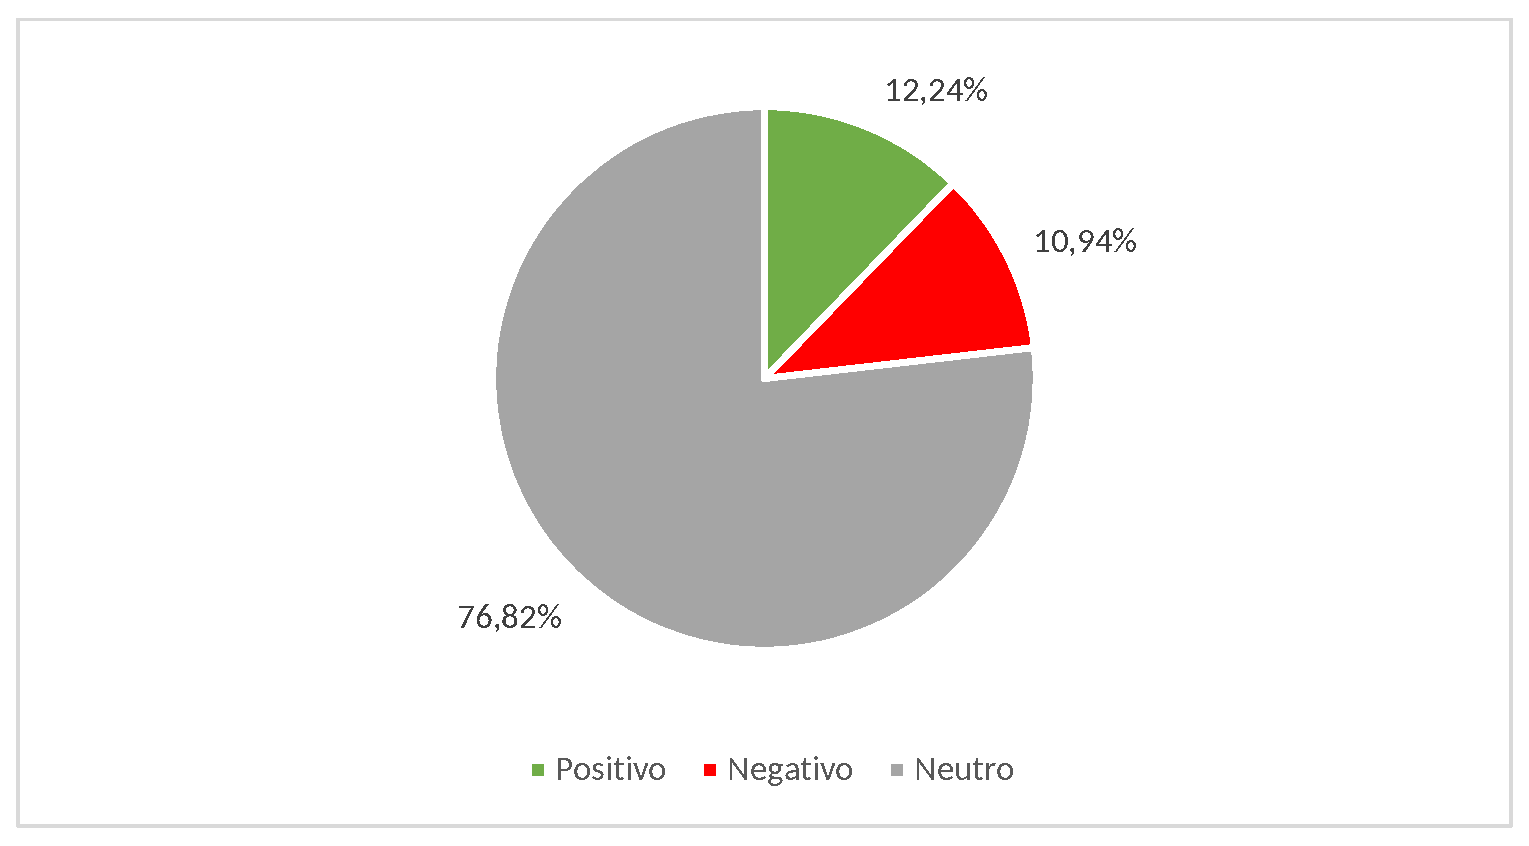
\epsfig{file=figuras/teste-1.eps, width=10cm}
	\caption{Quantidade de tweets separados por polaridade do teste 1. Fonte: Própria}
	\label{teste-graf-1}
\end{figure}

Nota-se que a quantidade de \textit{tweets} neutros é elevada, evidenciando que o modelo ainda tem dificuldade de definir a polaridade do texto. Com base nos resultados apresentados foram realizadas as seguintes mudanças visando diminuir a ocorrência de dados neutros.
 
\todo{Tabela 2 aqui}

Como mostra a tabela \ref{teste-2} as mesmas bases foram utilizadas, porém com a aplicação da técnica de \textit{stemming}, como  PUC-Stem e Sentilex-Stem. Além de utilizar a mesma técnica nas  \textit{stopwprds}. O resultado de 141.798 \textit{tweets}, 49.263 foram positivos, 35.079 negativos e 57.456 neutros.

\begin{table}[]
	\caption{2º teste}
	\label{teste-2}
	\resizebox{\textwidth}{!}{%
		\begin{tabular}{|l|l|r}
			\hline
			\multicolumn{3}{|c|}{2º Teste} \\ \hline
			\multicolumn{2}{|l|}{Bases usadas} & \multicolumn{1}{r|}{Tecnicas usadas} \\ \hline
			\multicolumn{2}{|c|}{Sentilex-Stem} & \multicolumn{1}{c|}{Stopwords} \\
			\multicolumn{2}{|c|}{PUC-Stem} & \multicolumn{1}{c|}{Stemming} \\ \cline{3-3} 
			\multicolumn{2}{|c|}{ReLi-Stem} &  \\ \hline
			\multicolumn{3}{|c|}{Resultado} \\ \hline
			\multicolumn{2}{|l|}{Positivo} & \multicolumn{1}{r|}{49.263} \\ \hline
			\multicolumn{2}{|l|}{Negativo} & \multicolumn{1}{r|}{35.079} \\ \hline
			\multicolumn{2}{|l|}{Neutro} & \multicolumn{1}{r|}{57.456} \\ \hline
			
		\end{tabular}%
	}
\end{table}

Analisando o 2º teste é visto que a quantidade de neutro diminuiu consideravelmente, apenas aplicando a técnica de \textit{stemming} nas bases de palavras.
\todo{grafico 2}
\begin{figure}[!h]
	\centering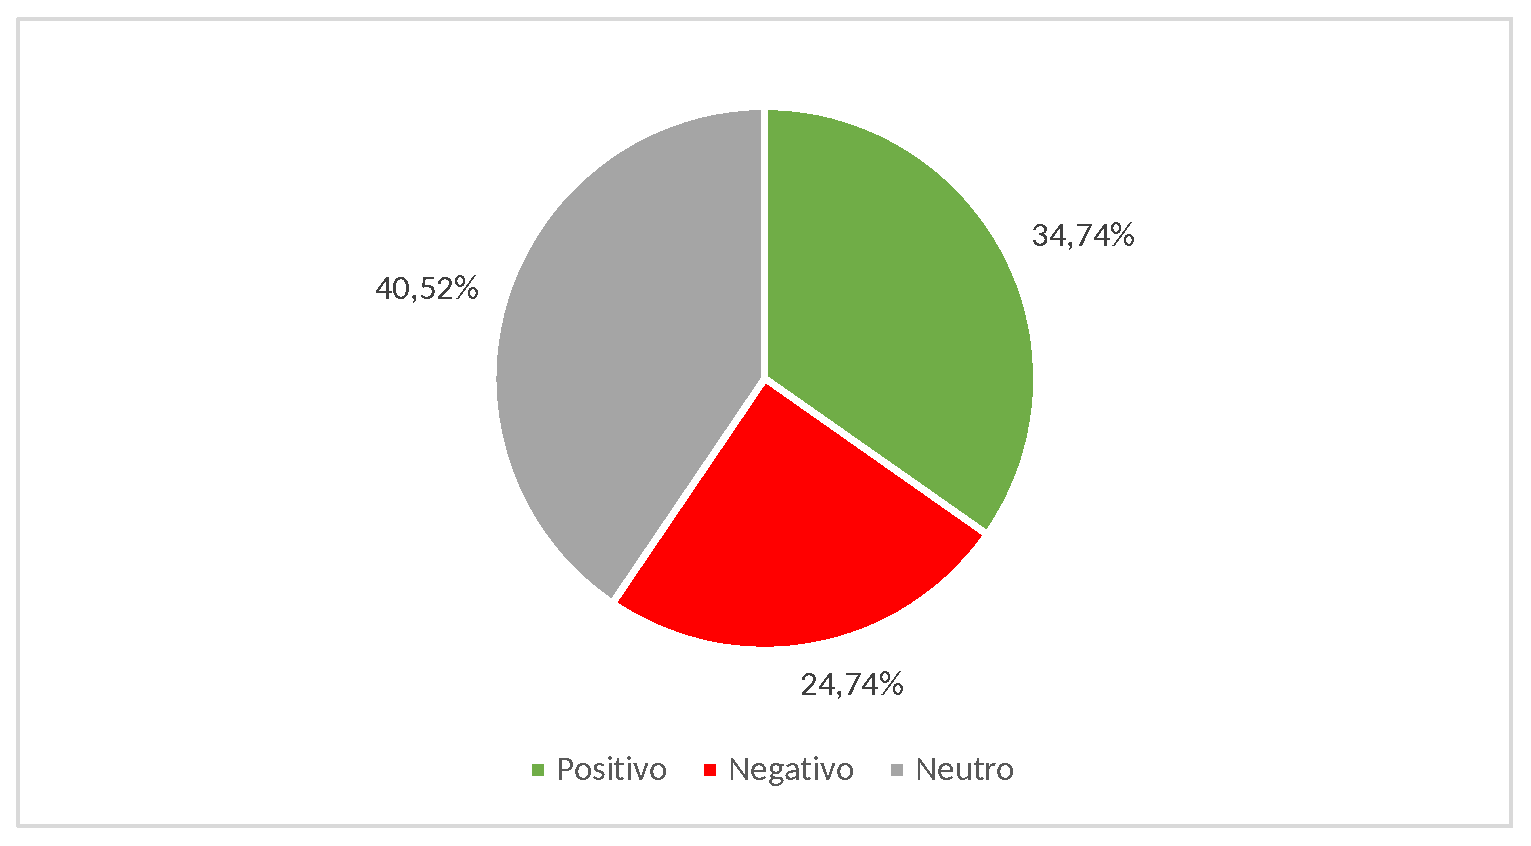
\epsfig{file=figuras/teste-2.eps, width=10cm}
	\caption{Quantidade de tweets separados por polaridade do teste 2. Fonte: Própria}
	\label{teste-graf-2}
\end{figure}

Ainda buscando a diminuição de dados neutros foi criada uma base de palavras mais próxima do domínio que esse trabalho propõe com a base chamada Oscar2016, essa base contém palavras relevantes ao evento, gerando o seguinte resultado.
\todo{colocar tabela 3 aqui}

\begin{table}[]
	\caption{3º teste}
	\label{teste-3}
	\resizebox{\textwidth}{!}{%
		\begin{tabular}{|l|l|r|}
			\hline
			\multicolumn{3}{|c|}{3º Teste} \\ \hline
			\multicolumn{2}{|l|}{Bases usadas} & Técnicas usadas \\ \hline
			\multicolumn{2}{|c|}{Oscar2016} & \multicolumn{1}{c|}{\textit{Stopwords}} \\ \hline
			\multicolumn{3}{|c|}{Resultado} \\ \hline
			\multicolumn{2}{|l|}{Positivo} & 47.450 \\ \hline
			\multicolumn{2}{|l|}{Negativo} & 7.210 \\ \hline
			\multicolumn{2}{|l|}{Neutro} & 87.138 \\ \hline
		\end{tabular}%
	}
\end{table}


Analisando a tabela \ref{teste-3} é visto que apenas uma base mais especializada no domínio não consegue diminuir a quantidade de neutros. O resultado de 141.798 \textit{tweets}, 47.450 foram positivos, 7.210 negativos e 87.138 neutros.


\todo{grafico 3}
\begin{figure}[!h]
	\centering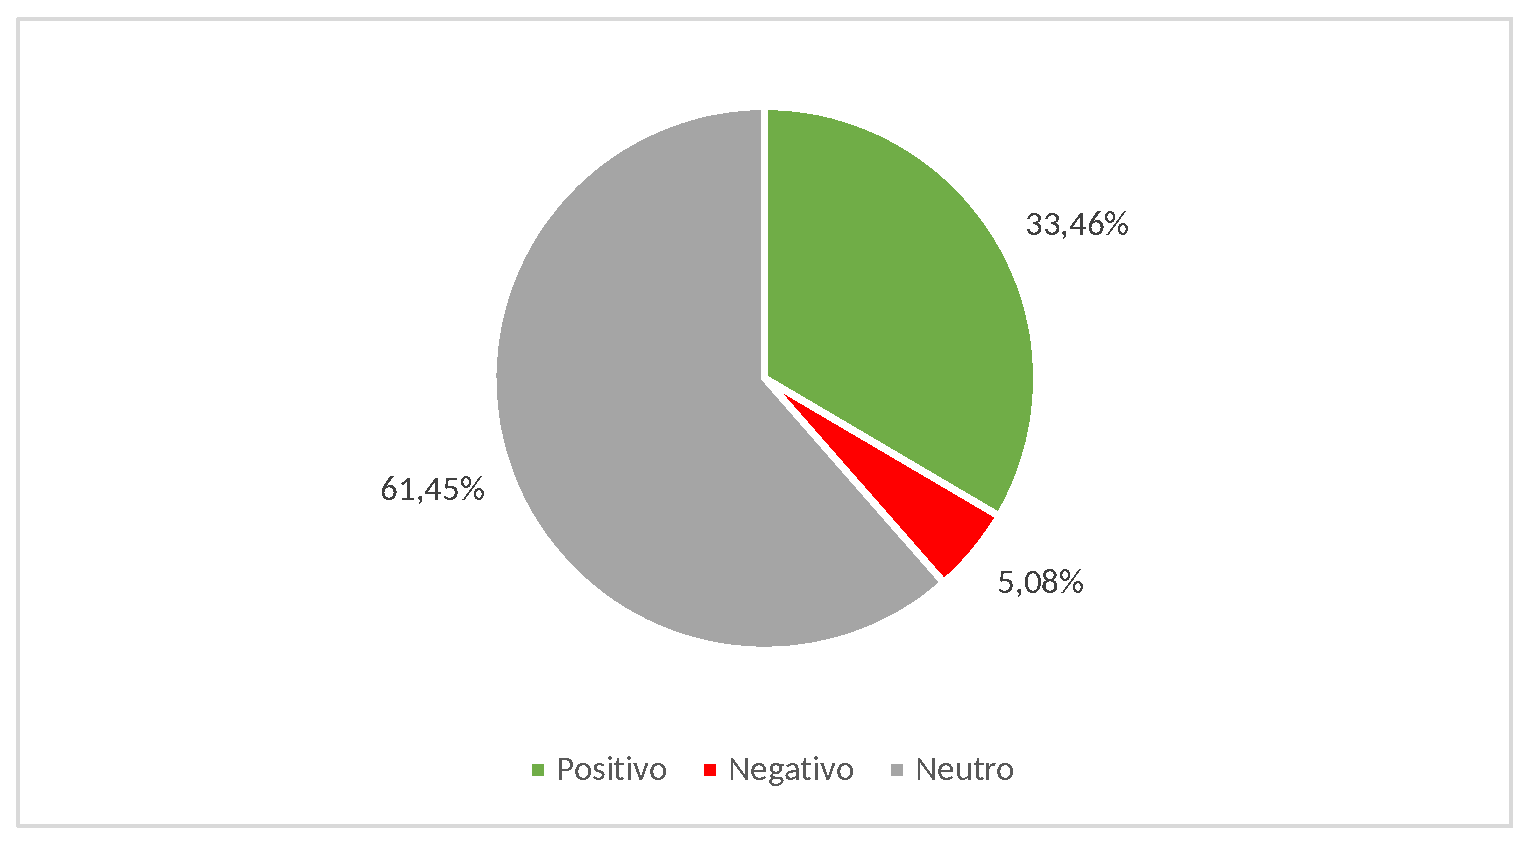
\epsfig{file=figuras/teste-3.eps, width=10cm}
	\caption{Quantidade de tweets separados por polaridade do teste 3. Fonte: Própria}
	\label{teste-graf-3}
\end{figure}

No 4º teste foi adicionada a base criada, Oscar2016 com as bases genéricas, Sentilex, PUC e  Reli  gerando o seguinte resultado:
\begin{table}[]
	\caption{4º teste}
	\label{teste-4}
	\resizebox{\textwidth}{!}{%
		\begin{tabular}{|c|l|r}
			\hline
			\multicolumn{3}{|c|}{4º Teste} \\ \hline
			\multicolumn{2}{|l|}{Bases usadas} & \multicolumn{1}{r|}{Técnicas usadas} \\ \hline
			\multicolumn{2}{|c|}{Oscar2016} & \multicolumn{1}{c|}{Stopwords} \\
			\multicolumn{2}{|c|}{SentiLex} & \multicolumn{1}{c|}{Stemming} \\ \cline{3-3} 
			\multicolumn{2}{|c|}{PUC} & \multicolumn{1}{c}{} \\
			\multicolumn{2}{|c|}{ReLi} & \multicolumn{1}{c}{} \\ \hline
			\multicolumn{3}{|c|}{Resultado} \\ \hline
			\multicolumn{2}{|l|}{Positivo} & \multicolumn{1}{r|}{69.070} \\ \hline
			\multicolumn{2}{|l|}{Negativo} & \multicolumn{1}{r|}{33.461} \\ \hline
			\multicolumn{2}{|l|}{Neutro} & \multicolumn{1}{r|}{39.267} \\ \hline
		\end{tabular}%
	}
\end{table}


Analisando a tabela \ref{teste-4} é visto que nesse teste foi obtido a maior taxa de diminuição de dados neutros. O resultado de 141.798 \textit{tweets}, 69.070 foram positivos, 33.461 negativos e 39.267 neutros.



\todo{Adicionar grafico 4}
\begin{figure}[!h]
	\centering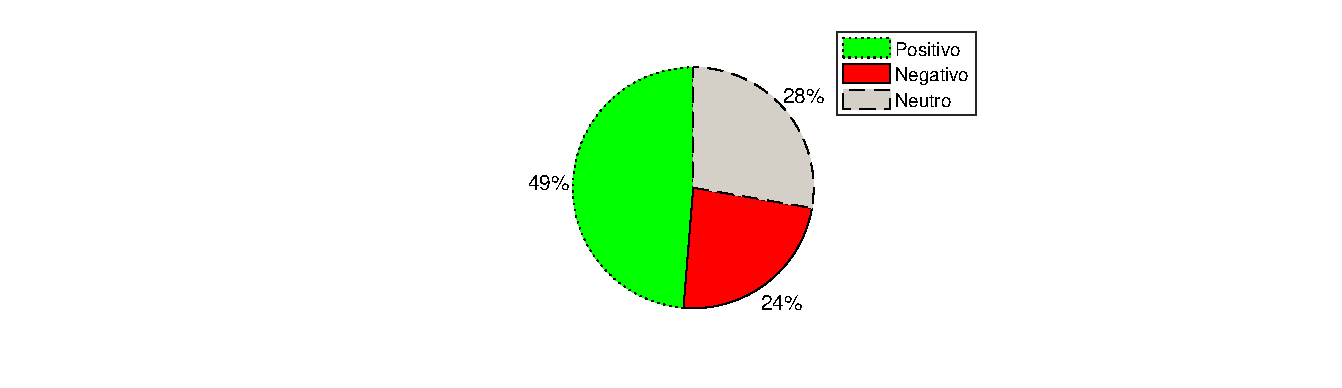
\epsfig{file=figuras/teste-4.eps, width=10cm}
	\caption{Quantidade de tweets separados por polaridade do teste 4. Fonte: Própria}
	\label{teste-graf-4}
\end{figure}
Segue abaixo um comparativo dos testes.

\begin{table}[]		
	\caption{Comparando testes}
	\label{teste-comp}
	\resizebox{\textwidth}{!}{%
		\begin{tabular}{l|l|c|l|l|}
			\cline{2-5}
			\multicolumn{1}{c|}{} & \multicolumn{1}{c|}{Teste 1} & Teste 2 & \multicolumn{1}{c|}{Teste 3} & \multicolumn{1}{c|}{Teste 4} \\ \hline
			\multicolumn{1}{|l|}{Positivo} & 15.517 & \multicolumn{1}{r|}{49.263} & 47.450 & 69.070 \\ \hline
			\multicolumn{1}{|l|}{Negativo} & 17.350 & 35.079 & 7210 & 33.461 \\ \hline
			\multicolumn{1}{|l|}{Neutro} & 108.931 & \multicolumn{1}{l|}{57.456} & 87.138 & 39.267 \\ \hline
		
		\end{tabular}%
	}
\end{table}

\begin{figure}[!h]
	\centering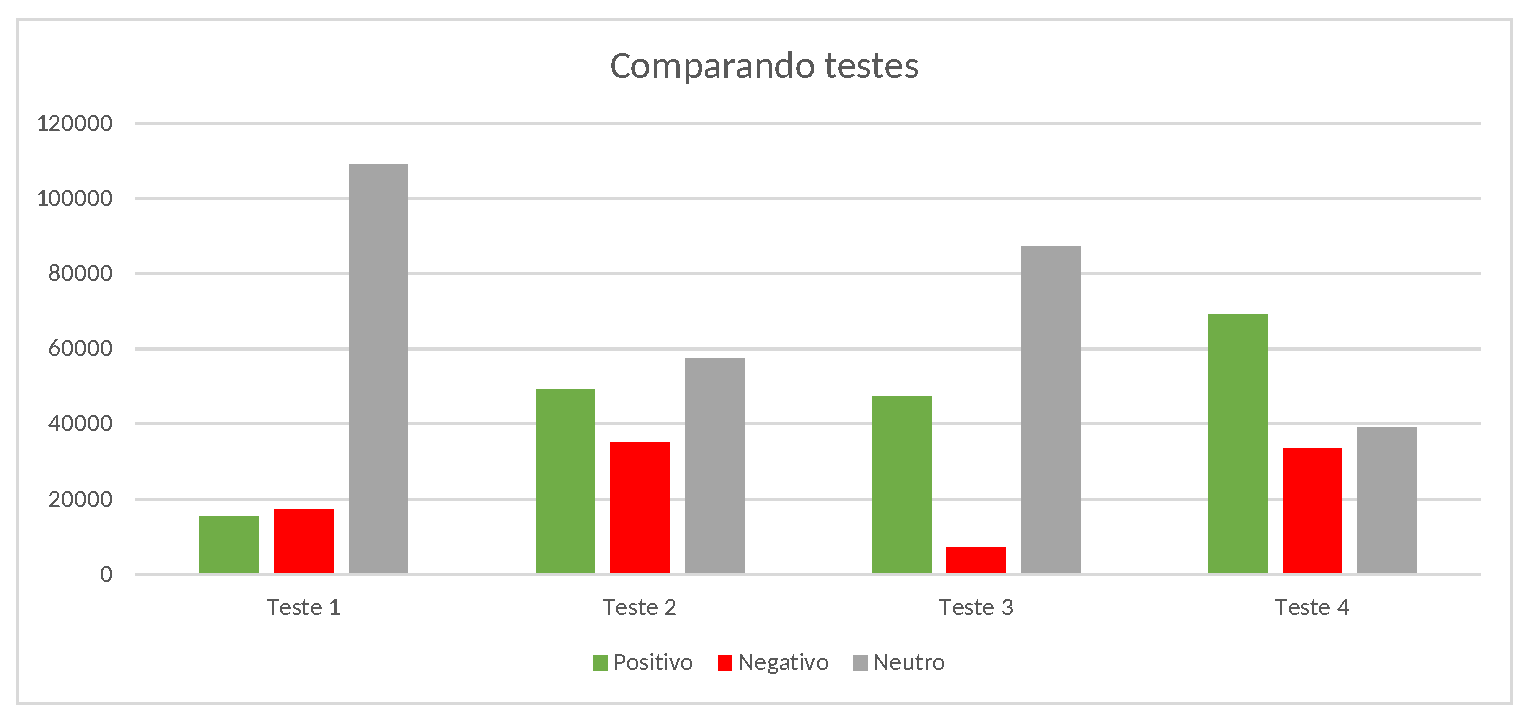
\epsfig{file=figuras/Pasta1.eps, width=15cm}
	\caption{Gráfico de comparação dos testes}
	\label{teste-graf-comp}
\end{figure}


Com o comparativo analisado na tabela \ref{teste-comp} foram escolhidas as configurações utilizadas no teste 4 para a realização da análise na base capturada, devido a menor presença de dados neutros classificados na base comprovando que as técnicas de \textit{stemming} e \textit{stopwords} foram válidas e relevantes para a sustentação modelo.

\section{Resultados}\label{result}

Para a análise dos resultados é necessário estabelecer premissas. O evento Oscar 2016 foi a  88.ª cerimônia de entrega dos \textit{Academy Awards} em \textit{Los Angeles}, Estados Unidos. O evento teve duração de aproximadamente 4 horas com seu início na noite do dia 28 de fevereiro, as 20:00 horário de Brasília no tapete vermelho com a entrada dos artistas e convidados. Seu encerramento as 2:00 do horário de Brasília do dia 29 de Fevereiro com a premiação do melhor filme. Os marcos do evento foram considerados: as entregas dos prêmios de cada categoria, o homenagem em memória póstuma e a apresentação da Lady Gaga e o discurso do Vice Presidente Americano. Esses eventos  são listados em ordem cronológica de acordo com a imagem \ref{time}

\begin{figure}[!h]
	\centering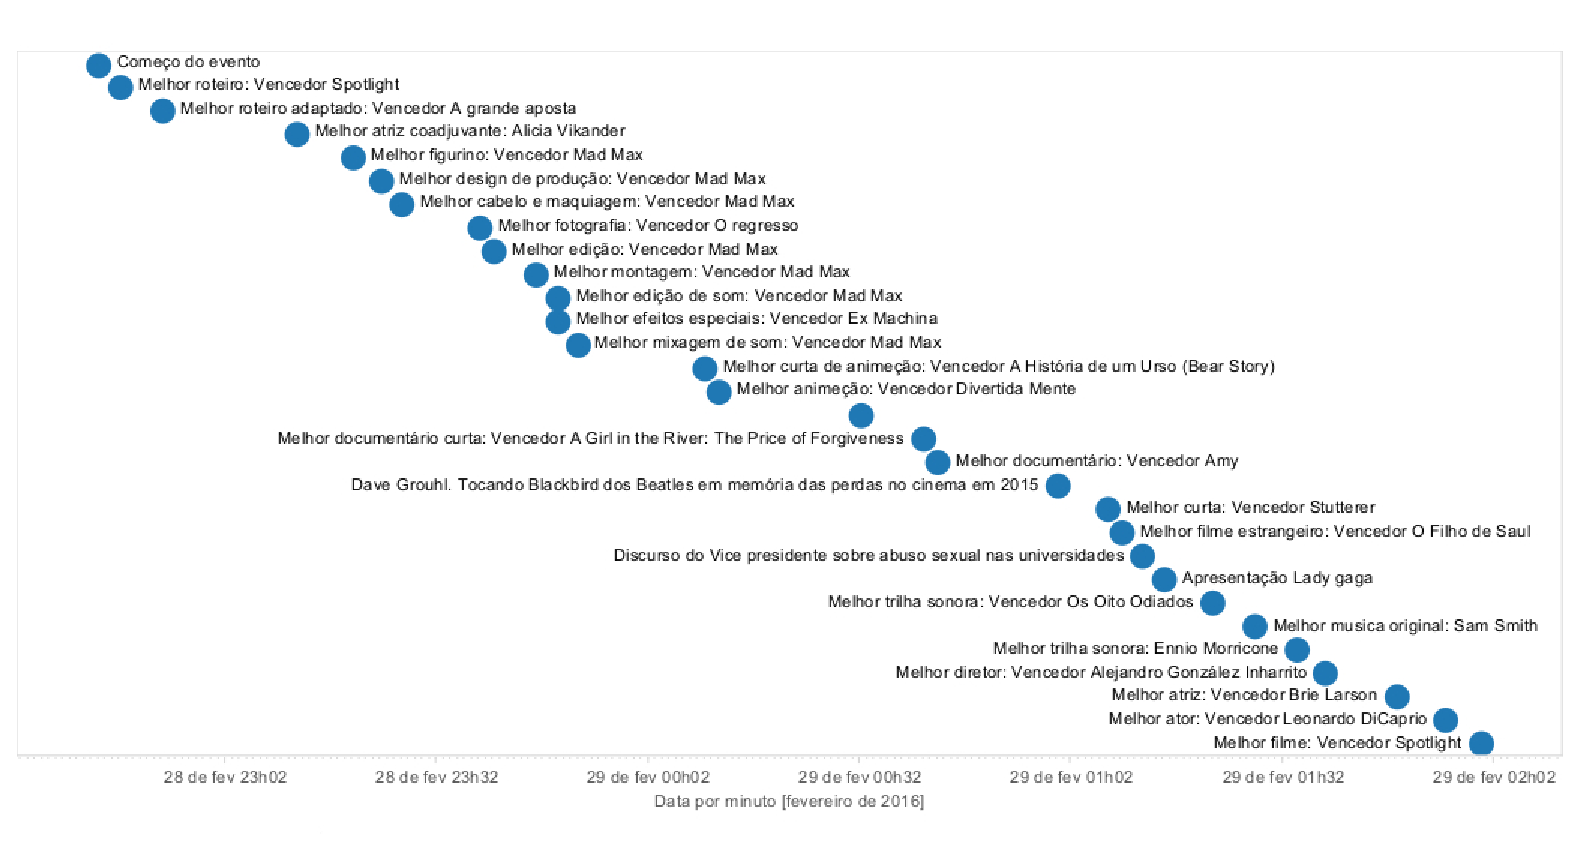
\epsfig{file=figuras/oscar_timeline.eps, width=15cm}
	\caption{Linha do tempo com os marcos do Oscar 2016. Fonte:Folha de São Paulo}
	\label{time}
\end{figure}
O gráfico \ref{qtd} mostra a curva da quantidade de \textit{tweets} em relação ao tempo  dividido pela polaridade. Nele é visto um pico  no começo do evento, durante o tapete vermelho, nesse período foi visto as maiores ocorrências de especulações sobre os ganhadores e indicados além das reações dos internautas com as entradas de seus artistas favoritos.

\begin{figure}[!h]
	\centering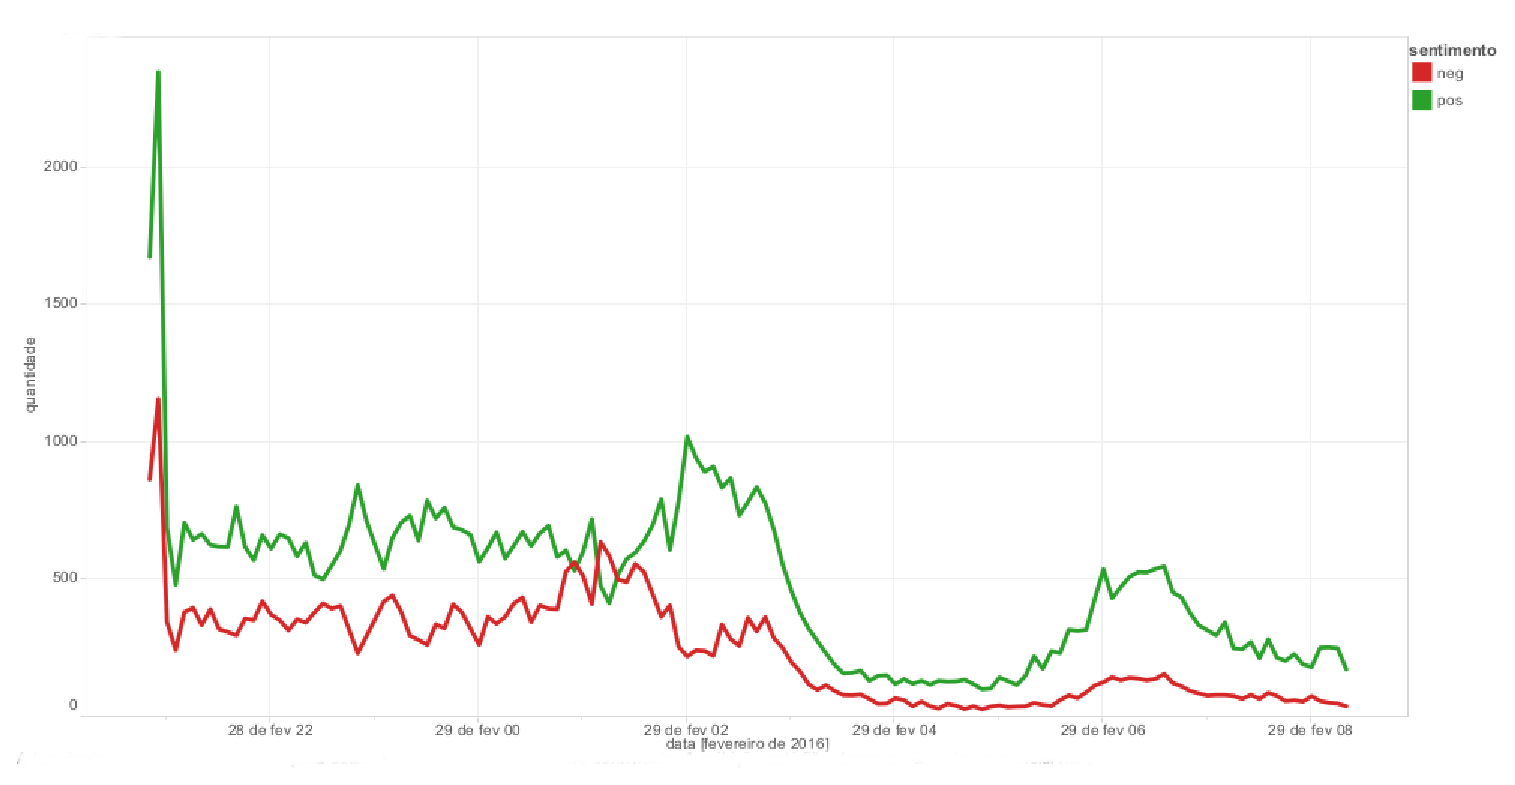
\epsfig{file=figuras/qtd_tweets_by_date.eps, width=15cm}
	\caption{Quantidade de tweets por tempo e polaridade. Fonte:Própria}
	\label{qtd}
\end{figure}

\begin{figure}[!h]
	\centering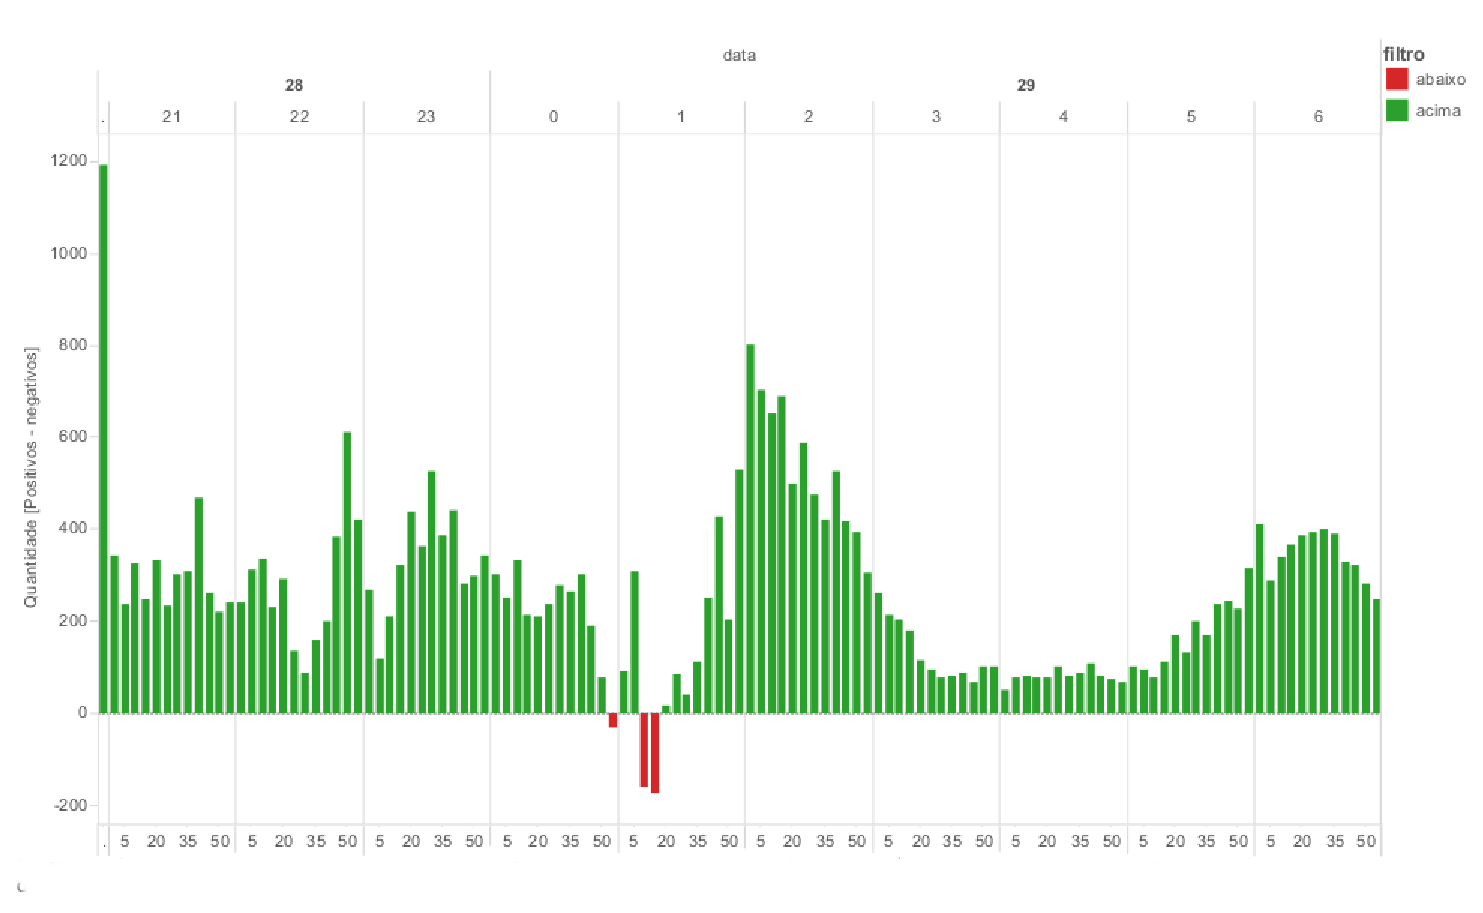
\epsfig{file=figuras/qtd_neg_pos.eps, width=15cm}
	\caption{Quantidade de tweets positivos diminuído pelos negativos pelo tempo. Fonte:Própria}
	\label{qtdnegpos}
\end{figure}

O gráfico \ref{qtdnegpos} foi gerado a partir da diminuição dos \textit{tweets} negativos pelos \textit{tweets} positivos vistos no gráfico \ref{qtd} produzindo uma visão micro do dados coletados do evento. Analisando o gráfico \ref{qtd}, que possui uma visão macro, junto com o gráfico \ref{qtdnegpos}, com a visão micro, é notado que em dois momentos a quantidade de \textit{tweets} negativos sobrepõem a quantidade de positivos. No primeiro momento, é durante o \textit{show} do Dave Grohl onde é feita uma homenagem aos falecidos no mundo do cinema em 2015 onde a sensação de luto ficou evidente durante a apresentação, e de acordo com \cite{freud1908conferencias}, é a reação à perda de objeto ou pessoa. Como afeto, o luto aproxima-se do humor depressivo. Com isso foi corroborado o aumento do sentimento negativo nessa parte do evento. Outro momento onde ocorre o mesmo efeito é durante a apresentação da Lady Gaga onde o tema do filme que a  música faz parte da trilha é sobre os estupros em faculdades americanas, e mais uma vez esse aumento negativo faz entender o tema pesado e sensível para as pessoas que sofreram e sofrem disso. Excluindo o pico no começo dos gráficos os maiores picos de positivos são presenciados as 2:00, vindo de uma crescente no final das 1:00 da manhã do dia 29 isso se deve as categorias mais aguardadas do evento que são:

 \begin{itemize}
 	\item Melhor atriz
 	\item Melhor ator
 	\item Melhor filme
 \end{itemize}

O maior destaque foi a premiação de melhor ator e a vitória de Leonardo DiCaprio, que com seus 41 anos de idade e 26 de carreira, nunca havia levado um prêmio de melhor ator da Academia. Essa vitória reflete nos gráficos de picos de positivos as 2:00 da manhã onde a repercussão da sua vitória é espelhada pelo twitter chegando aos \textit{trending topics} mundias na rede social.


\begin{figure}[!h]
	\centering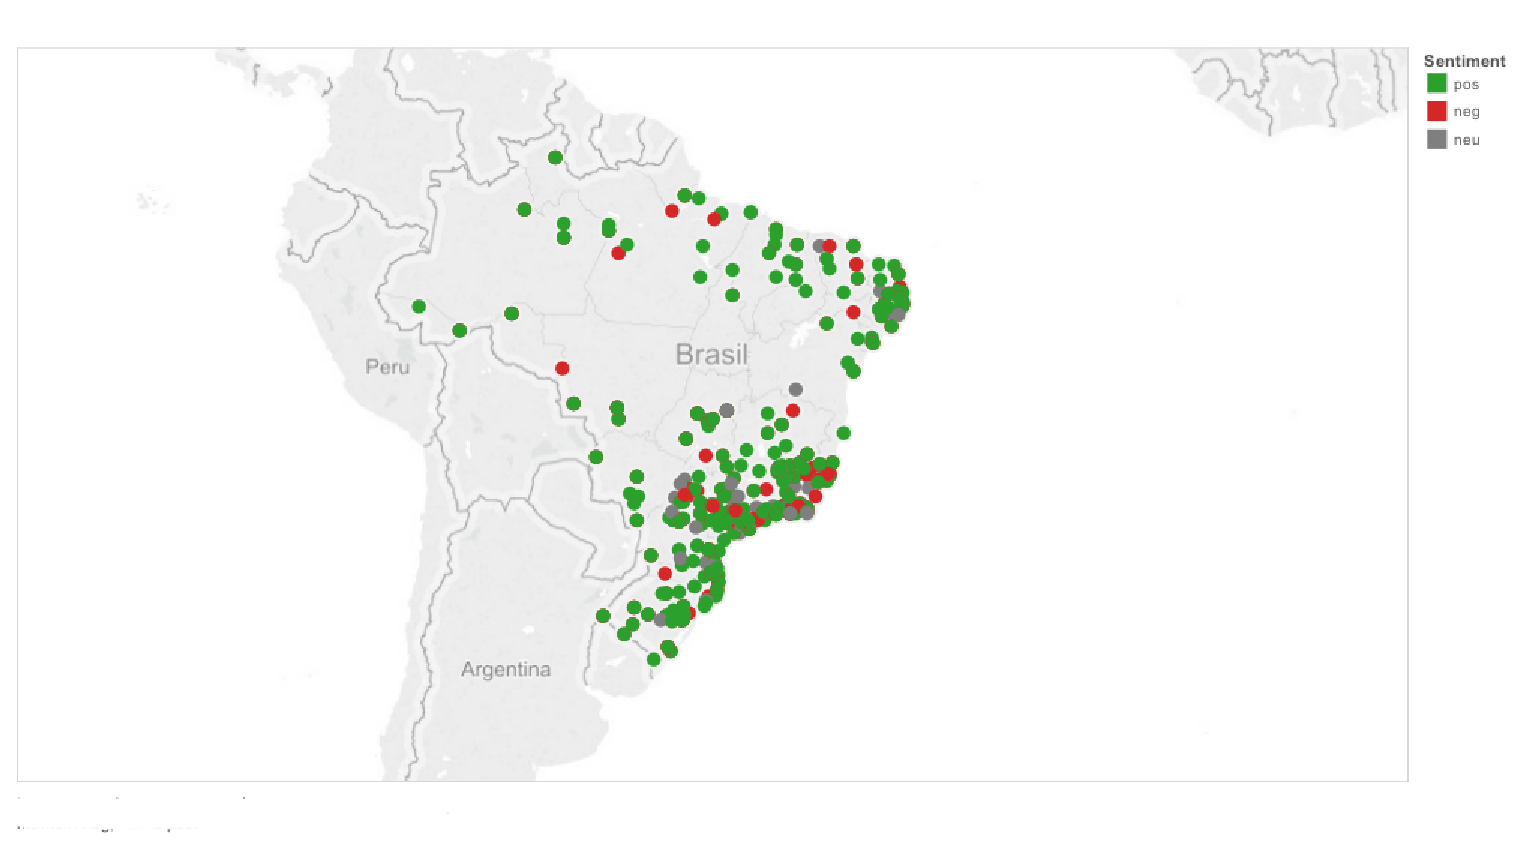
\epsfig{file=figuras/mapa.eps, width=15cm}
	\caption{Mapa de calor referente a polaridade de sentimento no Brasil. Fonte:Própria}
	\label{mapa}
\end{figure}